\part{Solution} \label{part:solution}

\chapter{Implementation}

This chapter will be the occasion to detail the architecture of our solution. We will explain the technologies employed to achieve our goal, a monitoring software for Internet of Things networks. It is also in this chapter that we will justify the choices we made during the development.

\section{Architecture}

The architecture of our solution is composed of two parts as can be seen on Fig.\ref{fig:design}. The first part is about how the data is collected and sent. The second part consists of how the data is received and treated after reception. In the remaining of this section, strong assumptions are made that the reader is familiar with Netflow, particularly IPFIX, also referred as Netflow v10, and also its implementation for WSN which is called TinyIPFIX. If not, explanations about those particular technologies can be found in Chap \ref{chap:monitoring_tools}. \\

\begin{figure}
	\centering
	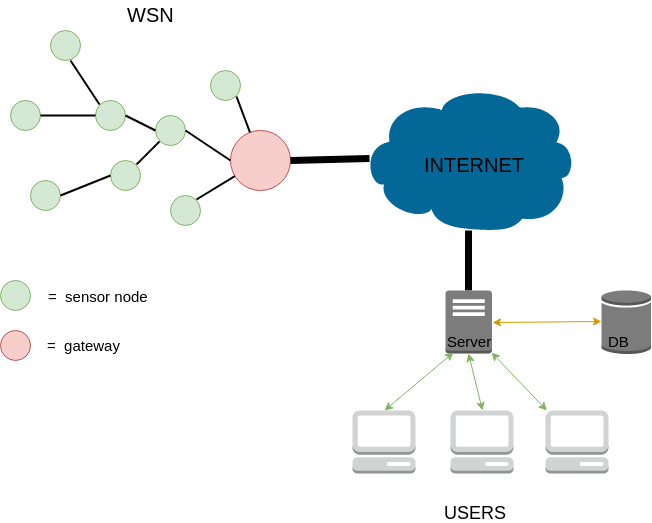
\includegraphics[width=0.8\textwidth]{res/design.png}
	\caption{Global architecture of the solution}
	\label{fig:design}
\end{figure}

The data exportation is done in a Netflow fashion. The nodes occupy the role of exporters. Each node maintains a flow table where they register the flows that occurred during an interval of time. In our case, a flow is characterized by the 4-uple: source node id, destination node id, number packets and number octets. After a certain amount of time, each node will construct a TinyIPFIX message based on the content of its flow table. Those messages are sent to the gateway node. The gateway node will then reformat the TinyIPFIX messages received into compliant IPFIX messages to a specific address, which will be in our case the address of a server. The messages are sent using UDP. It is not reliable but using TCP to transmit data would incur the cost of initiating the connection and closing it. Also in a reliable network with a high packet loss percentage, resending information would increase the load on the nodes.\\

The server that receives the IPFIX messages from the IoT network plays two roles. One role is straightforward, it is the the role of collector. Each message is collected by the server and logged in a database for further processing and analyze. The other role is of a web server. Multiple users can know the network status by having access to web pages served by the server.

\section{Technologies}

The monitoring tool developed for this thesis is a \textit{web-based} solution. We have chosen to write the monitoring tool with \textbf{Node.js} \cite{website:nodejs} which is a server-side solution for Javascript. In that sense, it offers modules or libraries to effectively develop HTTP server, i.e. a web server. To speed up our development, we used the \textit{Express framework} \cite{website:express} on top of Node.js. Express simplifies the routing of requests to views. A view can be seen as an web page. \\

The reasons we have chosen to write our monitoring tool as a web-server is the portability of such a solution. All OSs dispose of a web browser. For the user, it simplifies the utilization of the tool by simply accessing the web site via its preferred browser. The user does not have the trouble to download and install our software as with common desktop applications. Also, the user can freely access the tool from different locations or different computers. He is not limited to devices where the software is installed on. \\

Another factor in favor of a web solution is the ease with which multiple users can access the software at the same time. Most of the monitoring tools presented are desktop applications. They take the role of collectors and store the logs in a local database. This implies that the nodes transfer their data directly to the device having the monitoring tool on. However, a considerable drawback of such design is when multiple administrators exist for a same IoT network. Multiple users are bound to one device to monitor the network. One approach would be to retransmit the data sent by the nodes to each devices containing the monitoring tool in question, but it does not scale well. The web solution does not present that limitation. By having a centralized server playing the role of collector but also of web server, different users can efficiently monitor the network on their own device by simply requesting the web server. \\

One of the reasons for developing the software with Node.js and not other particular frameworks like Django or Ruby on Rails is due to the features that it offers via notably the Javascript language. First, it is event-driven and asynchronous by nature which is what we desire for our product. One such event to react to is when the collector receives an IPFIX message. Other events are for instance the status of a node changing as you will see later on. Programming by events proved to be powerful in our case. Secondly, the huge support on the Javascript language and its popularity which makes it a good choice for the adoption of the tool. Additionally, the huge documentations and modules helped us develop the tool faster and better. Thirdly but nonetheless, Javascript is tightly coupled to \acrfull{json} \cite{website:json} which is a data-interchange format. Objects in Javascript can be easily formated to JSON formated and exchanged via Internet. This allow to make dynamic website. Finally, we limit the language used during the process of production of the software mainly to Javascript for backend and HTML, CSS and Javascript for frontend where other frameworks would impose to master one or two more languages.\\

HTML, CSS and Javascript which are the core means to develop web pages proved to be useful but also easy to produce ways of visualizing the data. Javascript presents a lot of libraries to display graphs, charts and other type of figures. One such popular library is D3.js \cite{website:d3}. It also enables a website to be dynamic. Popular libraries like Bootstrap helped in making web page quicker and saved us the trouble to modify CSS files.\\

For the database, \textbf{PostgreSQL} \cite{website:postgresql} was used. It is an open-source relational database system. With more than 15 years of development, it does not have to prove anything anymore in term of reliability. It is SQL compliant. It recently added the support of JSON as field which enabled us to save IPFIX messages as JSON objects and not simply binary data.

\section{The monitoring tool}

This section will detail the different modules that compose our application plus the features that are offered by our application.

\subsection{Modules}

The application is comprised of four different modules :
\begin{itemize}
	\item Collector
	\item Log
	\item Nodes Status
	\item Web \\
\end{itemize}

The \textit{Collector} consists of a UDP server that listens to incoming IPFIX messages. Upon reception of a message, the Collector parses the binary data into an IPFIX object representing the original message. The object created is what will be used for the application to work with. It offers convenient methods to read records contained in the original IPFIX object. The Collector emits an event each time it creates an object from a received message. Modules can then listen and react to this particular event and treat the newly created object. \\

The \textit{Log} module offers logging capabilities of an IPFIX message. It also gives the possibility to query it. The storing is done in a PostgreSQL database. However, users can freely switch to its preferred SQL database as long as it also offers the possibilty to create a JSON field. To log an IPFIX message, it listens to the Collector's event mentioned before. It then stores in the database the JSON representation of the object. The module proposes methods to query the database such as having the different flows between two nodes as example. As to enhance the reactivity of our application, other tables are created apart from the ones that contained the IPFIX objects. One such table is the different flows.\\

To keep track of the status of the nodes, we deemed necessary to create a \textit{Nodes Status} module. This particular module also listens to the Collector's event for incoming IPFIX objects. It will then update the status of the nodes according to the content of the object. The status of a node comprises its parent, its battery, its number of bytes sent, number of packets sent and the last message sent, to name a few. The Nodes Status module offers the current state of the different nodes contained in the IoT network. To retrieve past values, it is necessary to pass via the Log module. The value of a status reflect the latest value received for that particular status. This means that if an IPFIX message contains the newest parent of the node, only the parent value of the node will be updated. The other status will remain the same.  \\

The final module is the \textit{Web} one. This module is essentially an HTTP server. Users interact with our tool mainly via this module. It permits users to visualize the status of their network via their browser by launching HTTP requests to which the server will reply by delivering the requested content. This module is an intermediate between the users and the Nodes Status module but also between the users and Log module. The reason for that is, to deliver content to the users, this module needs to gather data which is contained by the two aforementioned modules. This module can be seen as the frontend of our application whereas the other can be viewed as composing the backend of our solution.\\

The reasons behind using multiple modules is to achieve one of the requirements we imposed on ourselves, the \textit{modularity} of our program. We stated that a user should easily extend our software to add new features. By separating our applications into four different modules, we achieved this requirement. Each module offers different functionalities and abstractions. The Collector is responsible for collecting the IPFIX messages, the Log module to log those messages and provide means to query the logs, the Nodes Status keeps track of the status of the IoT network and finally the Web module permits users to interact and visualize the data. Users wanting to add new web pages will mostly only have to look into the Web module by adding another route to which the server will respond by replying by an HTML page. \\

The Fig.\ref{fig:modules} depicts the different modules presented and their interactions. As shown in the figure, the modules occupy different layers. The first layer is occupied by the Collector. The second one is occupied by the Nodes Status and Log modules. And finally, the third one is solely composed of the Web module. Those layers represent the level of interaction with the user with the top having the less interactions.

\begin{figure}
	\centering
	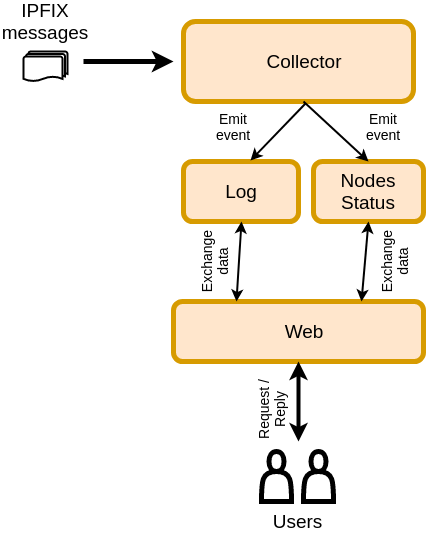
\includegraphics[width=0.5\textwidth]{res/modules.png}
	\caption{Modules interactions}
	\label{fig:modules}
\end{figure}

\subsection{Features}

The features offered by our monitoring applications are what we considered to be the basic ones. More description will be provided in the next chapter.

\begin{description}
	\item[Topology Map] Displays the logical topology of the WSN. The topology represents the RPL routing, meaning the topology is actually acyclic and represents a tree. A link represents a parent-child relation between two nodes. The root is the gateway node, and is colored differently to distinguish it from leaf nodes, which do not have children. Each node composing the topology is associated with its unique respective ID. Moreover, those nodes are uniquely clickable, one at a time, to get further information about their node values. Nodes are divided into three colors, i.e green, yellow and red, described their battery level.
	\item[Node values] Offers the possibility to see more in depth values sent by a particular node. With these features, an administrator has the possibility to see how the different values have evolved in time. It also gives meaningful statistics as the average number of bytes sent by interval of time, how often it is addressed and so on.
	\item[Network statistics] Gives statistics which are general to the whole network. This comprises the amount of traffic generated by the network. But also gives meaningful insight about the node having the lowest battery level or the node sending the most data. This gives a broad view to the administrator.
\end{description}

\chapter{The Monitoring Tool - A web interface}

In this chapter, we will showcase and explain the features of our Monitoring software. As stated earlier, we have built a web interface for the monitoring of IoT networks. There are two main tabs, one that showcases \textit{traffic volume} evolving through time, and the other one that shows the \textit{topology} of the IoT network under visualization.

\section{Traffic Volume}

The Traffic Volume page shows how the traffic has evolved through time for a particular network. As can be seen on Fig.\ref{fig:tool_traffic}, this page is divided into six different panels. \\

The first panel contains a graph that shows the evolution of the traffic in term of bytes over time. More precisely, we consider intervals of five minutes. This graph contains two lines. The blue one is for normal traffic and the other one in orange is for IPFIX traffic. Normal traffic is all the traffic that is not Ipfix nor TinyIPFIX. With that, administrators can see if the bytes generated by the monitoring with TinyIPFIX is of great importance or not. \\

The second panel, top right, is a brief summary of the network. It shows how much bytes and packets were sent. But it also shows the average packet size. Those number are computed for three type of traffics: IPFIX/TinyIPFIX traffic, normal traffic and also normal plus IPFIX/TinyIPFIX traffic.\\

The third panel, bottom left, shows statistics about the IoT network. Those statistics are the minimum and maximum bytes generated for a particular interval. It also gives information about the average number of bytes sent by interval. Those statistics are only computed on normal traffic. Deduction is thus done on the IPFIX/TInyIPFIX traffic.\\

The fourth panel is a pie chart showing the distribution of the total traffic. It shows the distribution of the traffic between IPFIX messages, broadcast messages and unicast messages. Broadcast messages are often used in networking for networks to organize  themselves such as finding neighbors, assigning addresses or routing purposes. By showing the proportion of broadcast messages, administrators can have an idea about the amount of data used to form the RPL topology.\\

Finally, the fifth and sixth panels show the top five sources and top five destinations respectively. The top sources the nodes that sent the most data while the top destinations are the nodes that received the most bytes. It permits to quickly see if for example a node presents a too large number of bytes sent compared to other nodes, or if a node is contacted too often.

\begin{figure}
	\centering
	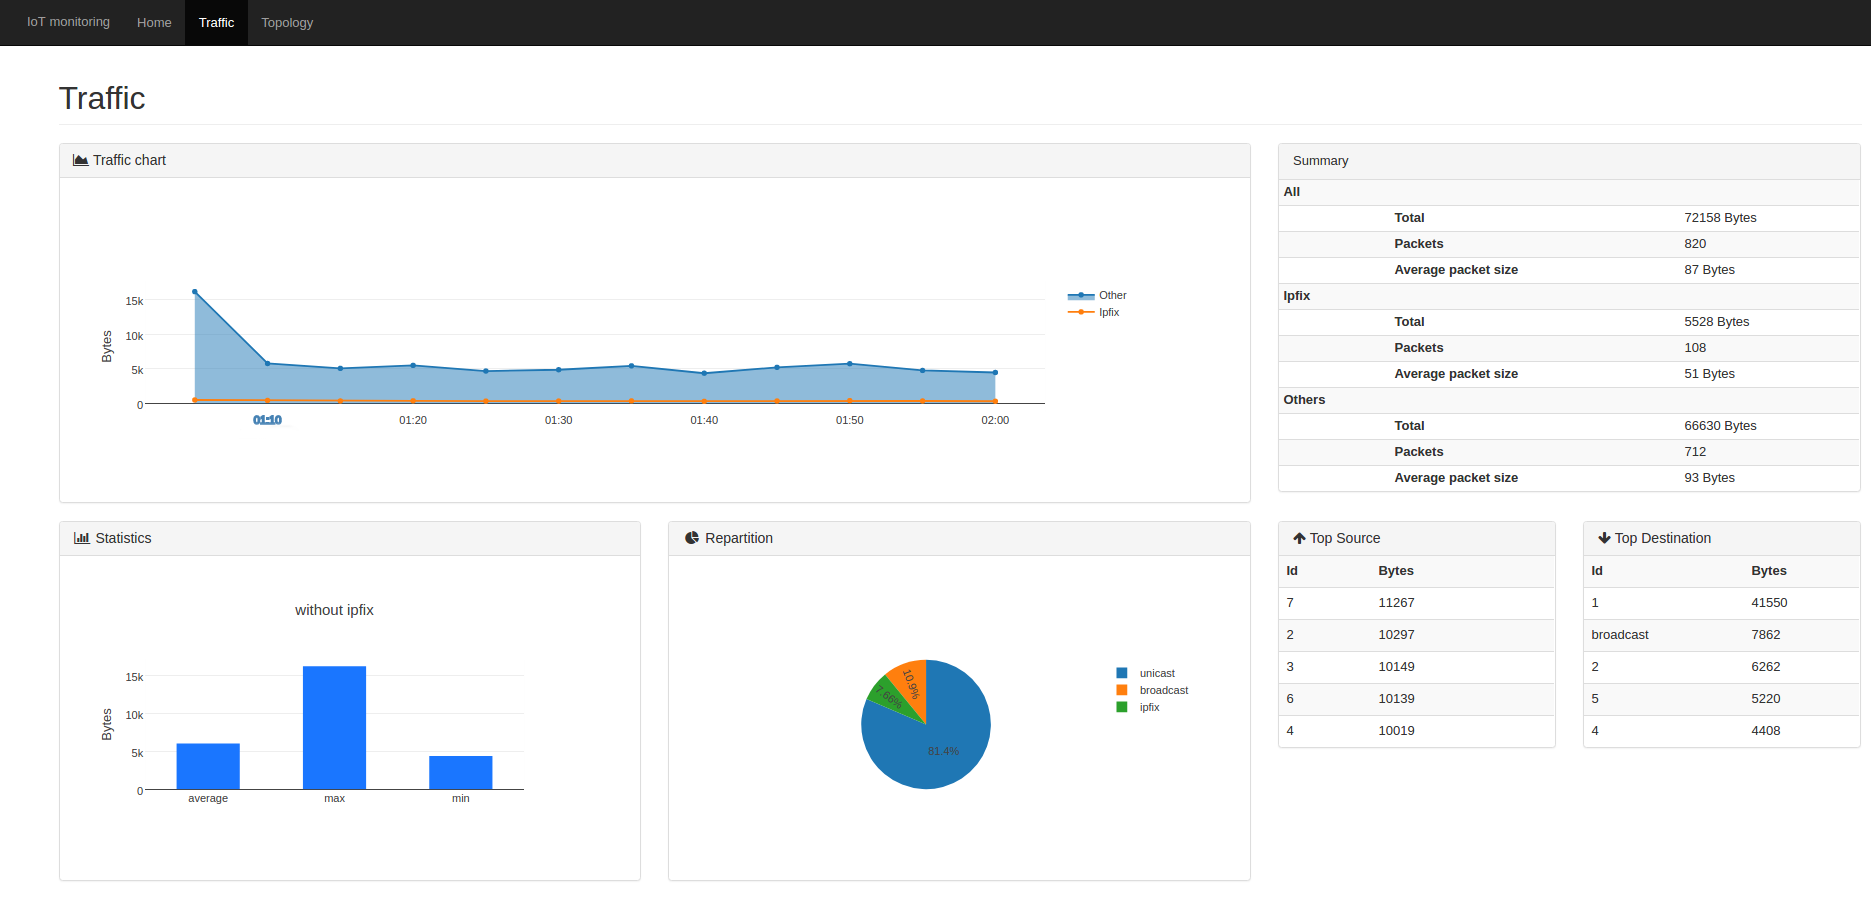
\includegraphics[width=\textwidth]{res/traffic.png}
	\caption{Traffic Volume}
	\label{fig:tool_traffic}
\end{figure}

\section{Current Topology}

\begin{figure}[!h]
	\centering
	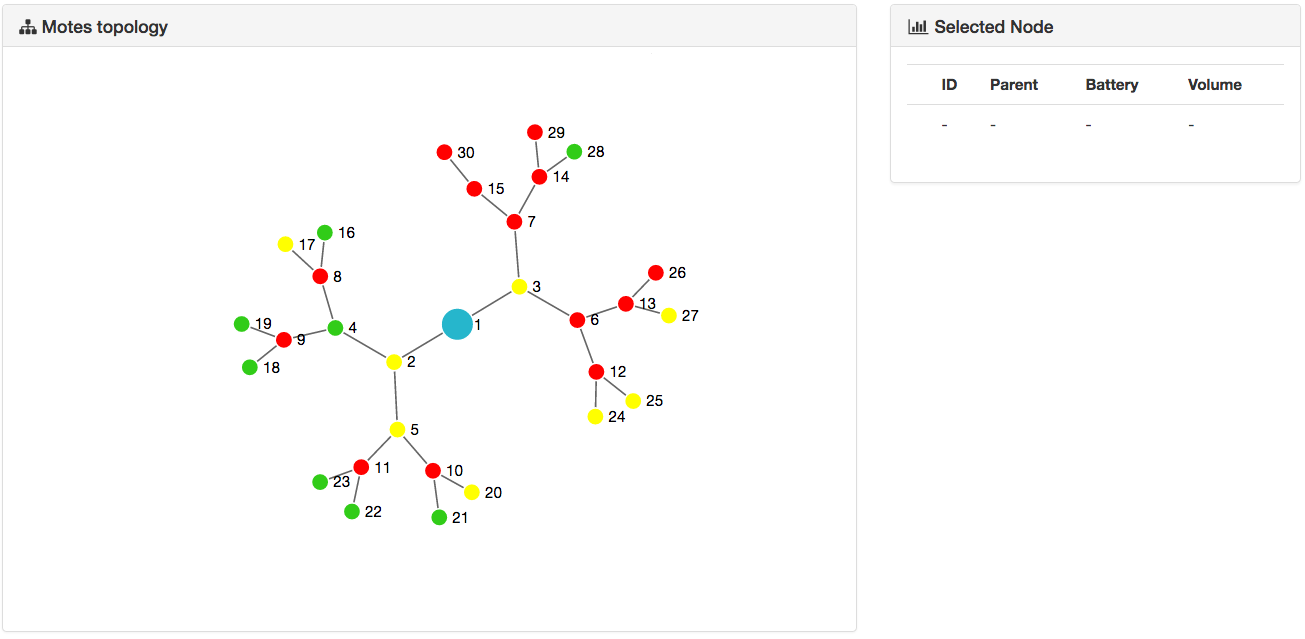
\includegraphics[width=1.1\textwidth]{res/topologyinterface.png}
	\caption{Topology Tab}
	\label{fig:topo}
\end{figure}

In this tab lies the topology of the network that is under visualization. Once all the traffic data has been received and processed by the server, it becomes possible to see the topology of our IoT network. As you can see in figure \ref{fig:topo}, the \textit{Motes topology} zone is where the graph is shown. \\

The traffic data used to build the topology is the last load of information received by the server from the IoT network. The gateway node forwards the IPFIX information collected by the nodes inside the network to the server which process it and update the routing topology. This is what mainly separate the Traffic Volume page from the Topology page. The Topology page is based only on the newest data while the other one use the logs stored in database. This page used only data provided by the \textit{Node Status} module explained in the chapter before.\\

It is worth noting that the topology is dynamic. Indeed, it reconstructs itself every time new information is received from the gateway node. However a refresh of the page is needed to see the modified topology. Hence, topology changes on the web interface are not made punctually. \\

Evidently, each node is represented as a circle, the \textit{gateway mote} being slightly larger and in sky blue. and each grey link represents a connection "parent to child" in the IoT network. All nodes in the topology are clickable, one at a time. It is not possible to click on a node if another node is already selected. Once a node is clicked on, its circle becomes larger and is filled in blue, as you can see in figure \ref{fig:snodeblue}. The \textit{Selected Node} panel (figure \ref{fig:snode} (either on the right or under the topology zone according to the browser's window size) allows to display specific information about the node we are interested in, namely its ID, its parent, its current battery level, and the total volume of data it has sent. The panel will use information based on the most recent messages received. Note that the Node \textbf{1} is the gateway mote of the network, it thus has no parent and its \textit{Parent} field is filled with "none", for other nodes it would contain another ID.\\

As for the three different colors for regular nodes, we have decided to use them as indicators for battery levels, a node in green has more than 50\% of battery, a node in yellow lies between 50 and 20, and a node in red is below 20\%. The colors could be used for other indicators in the network and with more tresholds, such as the total volume sent, or last time a node has sent information.\\

\begin{figure}[!h]
	\centering
	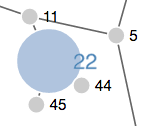
\includegraphics[width=0.6\textwidth]{res/snodeblue.png}
	\caption{Node clicked on}
	\label{fig:snodeblue}
\end{figure}


\begin{figure}[!h]
	\centering
	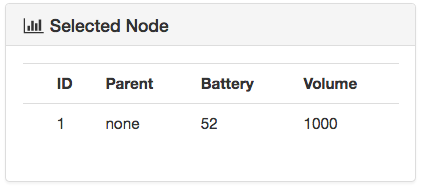
\includegraphics[width=0.6\textwidth]{res/snode.png}
	\caption{The panel showing specific data for a node}
	\label{fig:snode}
\end{figure}



\subsection{The Dragging feature}

\begin{figure}[!h]
	\centering
	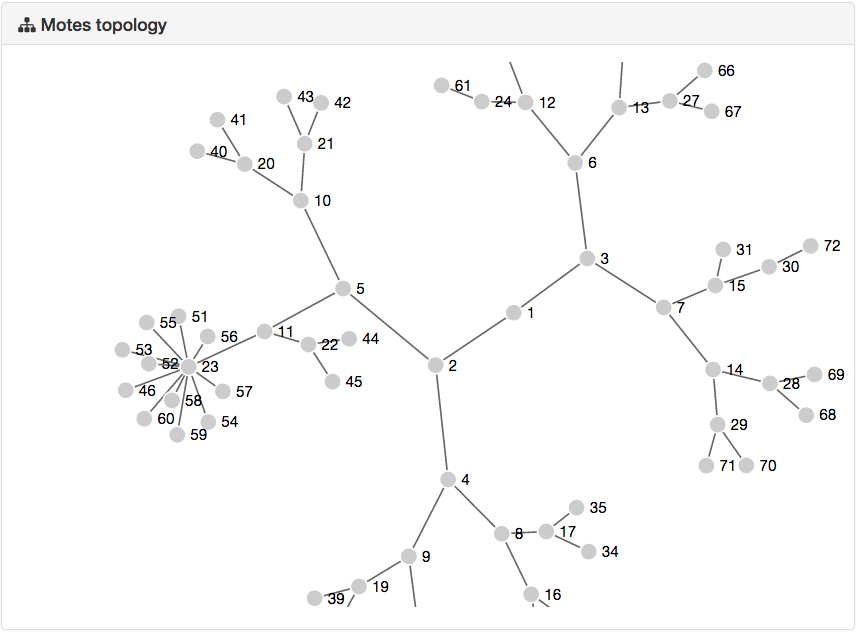
\includegraphics[width=0.6\textwidth]{res/populated.png}
	\caption{Populated topology, with out-of-border nodes}
	\label{fig:populated}
\end{figure}


We have decided to implement a dragging feature. That is, by clicking on a node and holding the click, it is possible to move the topology with the direction of the user's mouse. While this feature may seem insignificant, it finds its use when the topology gets populated. When there are more than 30 nodes (figure \ref{fig:populated}), the topology may expand further than the borders of the zone dedicated to the topology, as seen in figure \ref{fig:outnode}.\\



\begin{figure}
    \centering
    \begin{subfigure}[h]{0.3\textwidth}
        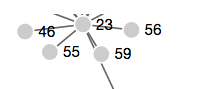
\includegraphics[width=\textwidth]{res/outnode.png}
        \caption{Out of borders nodes}
        \label{fig:outnode}
    \end{subfigure}
    ~
    \begin{subfigure}[h]{0.3\textwidth}
        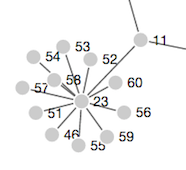
\includegraphics[width=\textwidth]{res/visible.png}
        \caption{Visible with dragging}
        \label{fig:visible}
    \end{subfigure}
    \caption{Dragging result}\label{fig:dragging}
\end{figure}

As you can see in figure \ref{fig:visible}, it is thus possible to fully see any group of nodes, since the topology zone is not unlimited in size. \\
